\documentclass{article}
\usepackage{amsthm, amsmath, graphicx, enumitem, tikz-qtree}
\usepackage[margin=0.5in]{geometry}
\graphicspath{ {7_img/} }
\begin{document}
    \noindent\textbf{CS 373 Homework 7}\hfill Anchu A. Lee\\
    \noindent\today\\
    \begin{enumerate}
        \item Construct a pushdown automata that recognizes $\{w \mid w $ is an element of $ \{0,1\}^* $ and $w$ has more 0's than 1's $ \}$.\\
        \begin{center}
            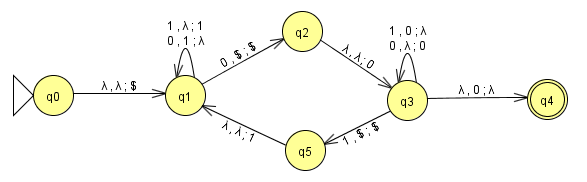
\includegraphics[scale=0.6]{machine1}
        \end{center}

        \item Convert the following CFG into an equivalent CFG in Chomsky normal form, using the procedure given in Theorem 2.9.
            \begin{align*}
                A&\rightarrow BAB\mid B\mid \epsilon\\
                B&\rightarrow 00 \mid \epsilon
            \end{align*}
            $S\rightarrow BC \mid AB \mid BA \mid BB \mid DD \mid \epsilon$\\
            $A\rightarrow BC\mid AB \mid BA \mid BB \mid DD$\\
            $B\rightarrow DD$\\
            $C\rightarrow AB$\\
            $D\rightarrow 0$
        \item Show that the class of context-free languages is closed under the union operation (construction and proof). The construction should be quite simple.
            \begin{proof}
                Define two context-free languages: $G_1=(V_1, \Sigma, R_1, S_2)$ and $G_2=(V_2, \Sigma, R_2, S_2)$ and also the language $G_U = (V_1\cup V_2\cup \{S\},\Sigma, R_1\cup R_2\cup \{S\rightarrow S_1 \mid S_2\}, S )$ which is the union of $G_1$ and $G_2$ as the start variable of $G_U$ points to both start variables of $G_1$ and $G_2$. Additionally the rules and variables are shared (assuming the rules and variables are disjoint). After the start variable of $G_U$, subsequent steps use rules exclusively from $G_1$ or $G_2$, not both. therefore all productions of $G_U$ must be in the languages $G_1$ or $G_2$.
            \end{proof}
        \item Show that the class of context-free languages is closed under the concatenation operation (construction and proof). The construction should be quite simple.

        \item Show that the class of context-free languages is closed under the star operation (construction and proof). The construction should be quite simple.

        \item Let $M=(Q,\Sigma, \delta, q_0, F)$ be a DFA and define CFG $G=(V,\Sigma,R,S$ as follows:
            \begin{itemize}
                \item $V = Q$;
                \item For each $q\in Q$ and $ a\in \Sigma $, define rule $q\rightarrow aq'$ where $q'=\delta(q,a)$;
                \item For $q\in F$ define rule $q\rightarrow\epsilon$;
                \item $S=q_0$.
            \end{itemize}
            Prove $L(M) = L(G)$.

        \item Let $L=\{0^n1^m0^n1^m \mid n,m \geq 0\}$. Show $L$ is not context-free.

        \item Let $L=\{w\mid w $ is in $\{a,b,c,d\}^*$, with the number of a's = number of b's and the number of c's = the number of d's $\}$. Show $L$ is not context-free.

        \item Let $A$ and $B$ be languages. We define $A\approx B = \{ab \mid a $ is an element of $A$ and $b$ is an element of $B$ and $|a| > |b|$ $\}$. Show that if $A$ and $B$ are regular languages, then $A\approx B$ is a context free language.

        \item Show $L = \{w\mid w $is an element of $\{a,b,c,d,e,f\}^*$ such that the number of a's + number of b's = number of c's + number of d's = number of e's + number of f's$ \}$ is not context-free.
    \end{enumerate}
\end{document}